\documentclass[a4paper, 12pt]{article}
\usepackage[utf8]{inputenc}
\usepackage{geometry}
\usepackage{polski}
\usepackage{graphicx}
\usepackage{float}
\usepackage{etoolbox,refcount}
\usepackage{multicol}

\newgeometry{left=2cm, right=2cm, bottom=2cm, top=1.5cm}

\begin{document}
	\begin{figure}[H]
		\centering
		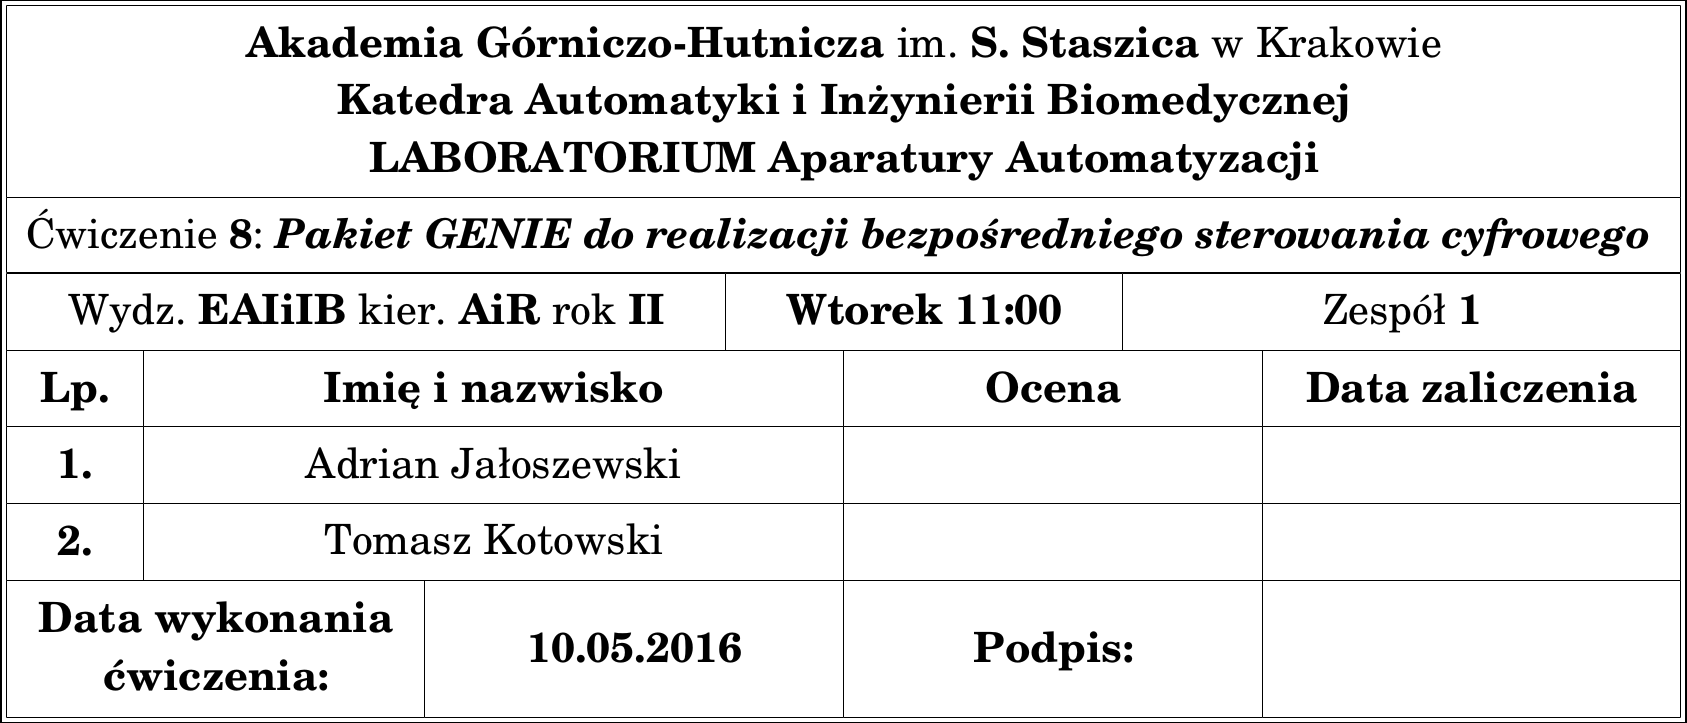
\includegraphics[width = \textwidth]{./img/cudo.png}
	\end{figure}
	\section{Cel ćwiczenia}
		Celem ćwiczenia jest zapoznanie się z przykładowym oprogramowaniem pozwalającym na realizację sterowania cyfrowego w oparciu o komputer klasy PC oraz zapoznanie się z przykładem interfejsu procesowego dla komputera klasy PC
	\section{Schemat stanowiska}
		Stanowisko składa się z komputera klasy PC z oprogramowaniem GENIE, połączonego ze stacją bazową ADAM5000. Do stacji są podłączone następujące moduły kontrolno pomiarowe:
		\begin{itemize}
			\item[--] ADAM5060 -- wyjścia cyfrowe -- podłączona lampa, którą sterujemy, gniazdo 0
			\item[--] ADAM5018 -- wejścia analogowe, podłączony czujnik natężenia światła, gniazdo 1
			\item[--] ADAM5013 -- wejścia termometru oporowego PT100, gniazdo 3
		\end{itemize}
		\begin{figure}[H]
			\centering
			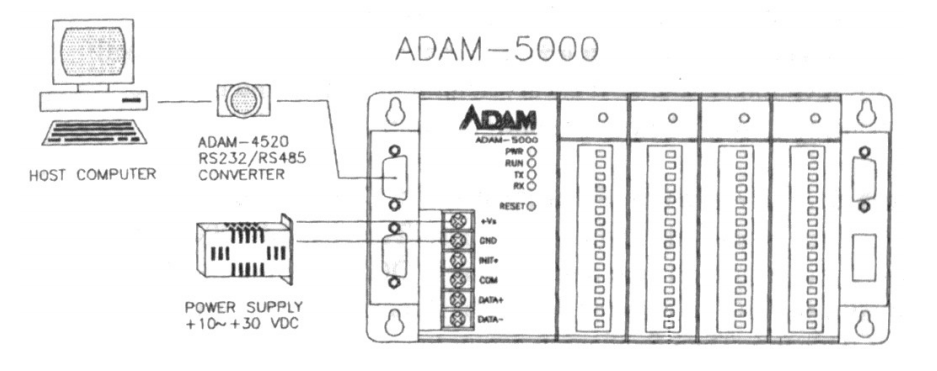
\includegraphics[width = \textwidth]{./img/adam.png}
		\end{figure}
	\section{Opis pakietu GENIE}
		Oprogramowanie GENIE pozwala na realizację bezpośredniego sterowania cyfrowego. Program obsługujący urządzenia zewnętrzne napisany w GENIE jest nazywany strategią, a pliki te posiadają rozszerzenie ,,.GNI''. GENIE jest programem graficznym, składającym się z następujących elementów:
		\begin{itemize}
			\item[--] TASK DESIGNER -- odpowiada za projektowanie aplikacji, graficzna reprezentacja potrzebnych funkcji
			\item[--] DISPLAY DESIGNER -- odpowiada za tworzenie graficznego interfejsu użytkownika
			\item[--] REPORT DESIGNER -- odpowiada za tworzenie szablonów raportów generowanych przez zaprojektowany przez nas system
			\item[--] SCRIPT DESIGNER -- służy do pisania skryptów
		\end{itemize}
		Aby uniknąć sytuacji, gdzie po wyłączeniu sterowania układ dalej pracuje albo rozpoczyna pracę bez odpowiednich ustawień oprogramowanie GENIE udostępnia możliwość napisania skrypów, które pełnią rolę konstruktora i destruktora -- jeden inicjuje układ przed jego uruchomieniem, \linebreak a drugi zakańcza jego działanie po wyłączeniu. Skrypty mogą być pisane w Visual Basic'u, wadą tego rozwiązania jest wolne wykonywanie się skryptu, gdyż musi zostać zinterpretowany. Oprócz tego można korzystać z plików DLL, które pozwalają na definiowanie własnych bloczków. 
	\section{Przeprowadzenie ćwiczenia}
		Ćwiczenie rozpoczęliśmy od zaprojektowania prostych strategii, których celem było sprawdzenie poprawności działania stanowiska. Była to strategia odpowiedzialna za włączanie lampy oraz strategia odpowiedzialna za pobieranie danych z czujnika natężenia światła i zaznaczania go na wykresie. Zauważyliśmy tu, że szybkość działania strategii jest zbyt mała i należy ją zwiększyć. Przy okazji zobaczyliśmy co się dzieje w przypadku jeżeli oprogramowanie działa szybciej niż jesteśmy w stanie pobierać dane.
		\subsection{Strategia}
			Po zapoznaniu się z praktycznym działaniem oprogramowania GENIE i sprawdzeniu, że wszystko poprawnie działa przystąpiliśmy do kolejnego kroku jakim jest skonstruowanie zaawansowanego wyłącznika zmierzchowego realizującego postawioną przed nami funkcjonalność. 
			\begin{figure}[H]
				\centering
				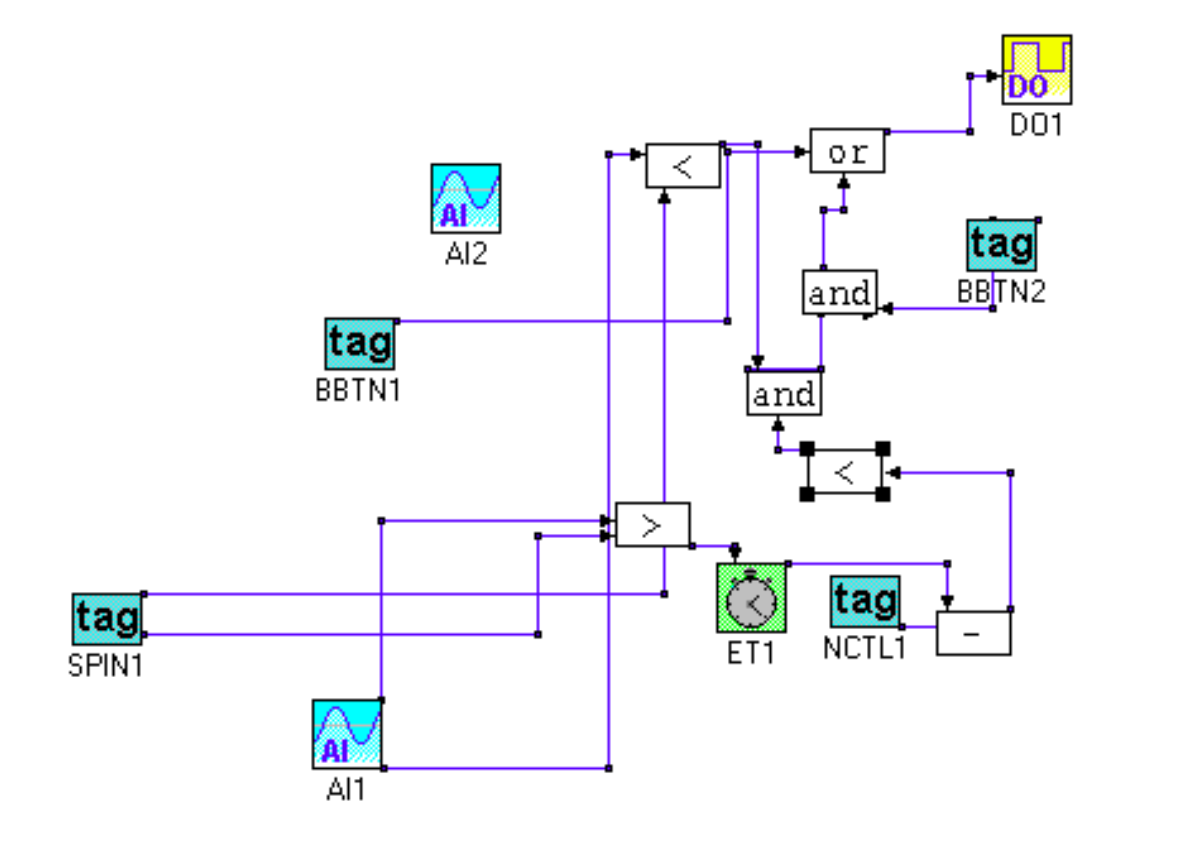
\includegraphics[width = 0.8\textwidth]{./img/schemat.png}
			\end{figure}
			\noindent Powyższa strategia realizuje postawione zadanie przy pomocy bloczków wejść analogowych, wyjścia cyfrowego, operacji logicznych, timera oraz komparatorów. Odpowiednie tagi są odpowiedzialne za:
			\begin{itemize}
				\item[--] BBTN1 -- nadrzędny włącznik lampy
				\item[--] BBTN2 -- blokada automatu
				\item[--] NCTL1 -- czas przez jaki ma być włączona lampa
				\item[--] SPIN1 -- wartość progowa poziomu oświetlenia
			\end{itemize}
			Wejścia analogowe i wyjście cyfrowe to odpowiednio:
			\begin{itemize}
				\item[--] AI2 -- wejście pomiaru temperatury
				\item[--] AI1 -- wejście pomiaru natężenia światła
				\item[--] DO1 -- wyjście na lampę
			\end{itemize}
		\subsection{Panel operatorski}
			Poniższa grafika przedstawia panel operatorski w stanie działania w chwili wykonywania testów, jakimi było przysłanianie dłonią czujnika poziomu oświetlenia i rejestrowanie zachowania układu w reakcji na to.
			\begin{figure}[H]
				\centering
				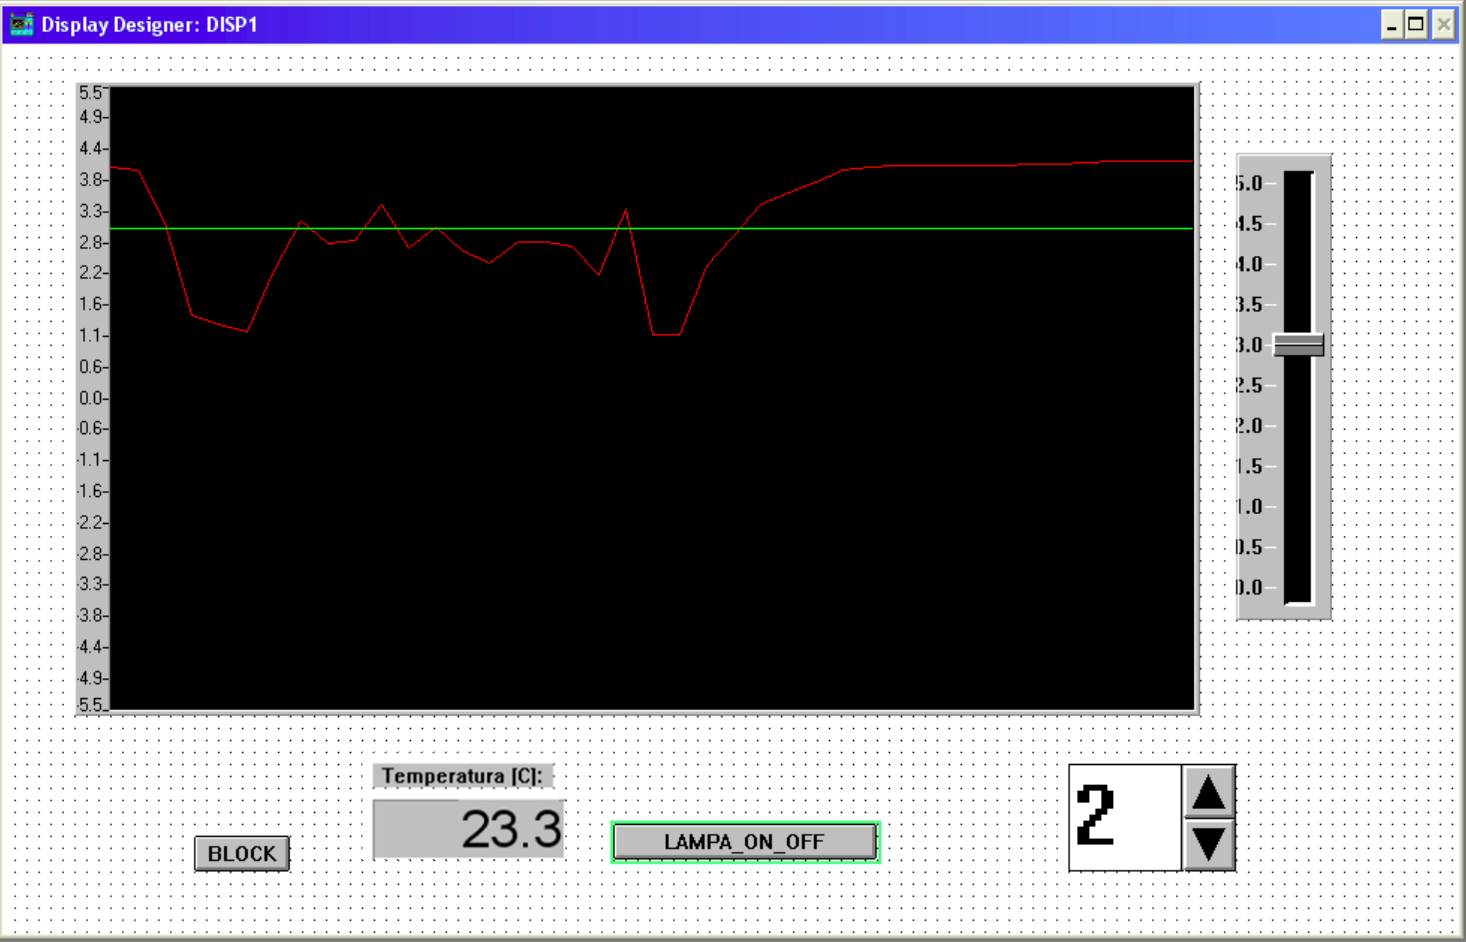
\includegraphics[width =\textwidth]{./img/przebieg.png}
			\end{figure}
			\noindent Na wyświetlaczu zielona linia przedstawia aktualną wartość progową ustaloną suwakiem na prawo od wyświetlacza, a czerwona linia przedstawia aktualny pomiar poziomu oświetlenia. Okienko do wprowadzania danych ustala czas włączenia lampy po zejściu aktualnego poziomu oświetlenia poniżej wartości progowej. Dwa przyciski odpowiadają za przełączanie lampy oraz za blokowanie automatu. Okienko z temperaturą pokazuje aktualną temperaturę pomieszczenia.
		\subsection{Opis strategii}
			Nadrzędny włącznik światła jest połączony alternatywą logiczną z automatem odpowiedzialnym za włączanie na pewien czas układu, gdyż jeżeli wtedy przyjmie wartość logiczną 1, to wyjście będzie 1, a w przeciwnym wypadku na wyjściu alternatywy pojawi się wyjście z automatu.
			\newline 
			\newline 
			Wyjście z automatu jest koniunkcją tagu odpowiedzialnego za blokowanie automatu oraz pozostałej części automatu. W ten sposób dla włączonego tagu przesyłany jest sygnał nadawany przez resztę automatu, a w przypadku wyłączonego tagu na wyjściu zawsze jest zero logiczne. Odwrotne działanie (wysoka wartość logiczna dla wyłączonej blokady) osiągnęliśmy przez zmianę w DISPLAY DESIGNER.
			\newline 
			\newline
			Jeżeli wejście z czujnika poziomu oświetlenia jest niższe od wartości progowej, to uruchamiany jest timer, którego wartość jest porównywana z czasem ustalonym w panelu operatorskim. Układ ten jest połączony koniunkcją z innym komparatorem ze względu na możliwość wzrostu poziomu oświetlenia ponad limit -- światło musi zgasnąć.
			\newline 
			\newline
			Wejście analogowe z termometru jest podłączone bezpośrednio do elementu odpowiedzialnego za wyświetlanie temperatury.
	\section{Wnioski}
		Cele ćwiczenia zostały zrealizowane mimo niewielkich trudności jakie mieliśmy z początku, gdyż musieliśmy uruchamiać system od nowa ze względu na wadę oprogramowania. Oprócz tego ćwiczenie przebiegło bez większych problemów.
		\newline
		\newline
		Zapoznaliśmy się ze standardem transmisji szeregowej RS-485, poznając jego zalety oraz wady, jak i topologie w jakie mogą być łączone przy pomocy jego odbiorniki. Dowiedzieliśmy się \linebreak o ograniczeniach tego standardu w stosunku do RS-232 oraz o jego przewadze nad niniejszym -- można przesyłać dane na większe dystanse.
		\newline 
		\newline
		Nauczyliśmy się korzystać z oprogramowania Genie oraz używaną w tym programie terminologią. Poznaliśmy zarazem kolejny język graficzny, pozwalający na szybkie projektowanie algorytmów. Wiemy jak korzystać z tego oprogramowania, jego budowę oraz wady i zalety takiego rozwiązania. Jest to środowisko zbyt wolne do wykonywania obliczeń czasu rzeczywistego w większych systemach ze względu na konieczność interpretowania skryptów oraz współpracę z systemem operacyjnym. Jest to jednak bardzo wygodne narzędzie do symulacji i prototypowania.
		\newline
		\newline
		Poznaliśmy serię urządzeń ADAM5000 wraz z niektórymi jego modułami i sposobem ich dołączania. Dowiedzieliśmy się jak można przy pomocy tych modułów dokonywać pomiarów oraz jak można wyprowadzać sygnały na wyjścia. Zaznajomiliśmy się z protokołami komunikacyjnymi wykorzystywanymi przez tę serię oraz z wykorzystywanymi standardami połączeń. 
\end{document}
